\chapter{ASP程序解释与调试系统的设计与实现}
\section{ASP程序解释与调试系统设计}
本文实现的ASP程序解释系统采用典型的三层架构式系统,分别为交互层、业务逻辑层以及数据层,每一层都包含不同的功能和数据模块,分模块对ASP程序的解释系统进行设计。图\ref{fig:exp_system}为ASP程序解释系统的系统结构示意图,下面将分别对图中的交互层、业务逻辑层以及数据层进行详细介绍。
\begin{figure}[htbp]
    \centering
    \includegraphics[width=\textwidth]{figures/解释系统结构.jpg}
    \caption{解释系统结构示意图}
    \label{fig:exp_system}
\end{figure}

\section{ASP程序解释与调试系统实现}
\subsection{系统环境与架构}
ASP程序的调试与解释系统基于 B/S 架构实现,采用RESTful架构实现,前后端分离。前端使用Web框架Angular-8.3.8实现,后端采用Spring Boot-2.2.6实现,同时使用了 HTML、JavaScript、JQuery等技术来对用户交互部分进行实现,ASP求解器使用Clingo 5.5.0,求解Well-founded Model时则使用dlv求解器,数据库采用Mysql 8.0.23,程序语法解析工具采用Antlr-4.8。开发系统的硬件配置为2 GHz,四核Intel Core i5,内存8.00GB,操作系统为 macOS BigSur 11.3,开发工具为 IntelliJ IDEA,IntelliJ Pycharm, Intellij Webstorm。
\subsection{运行界面}
\subsubsection*{1) 程序录入与求解}
\begin{figure}[htbp]
    \centering
    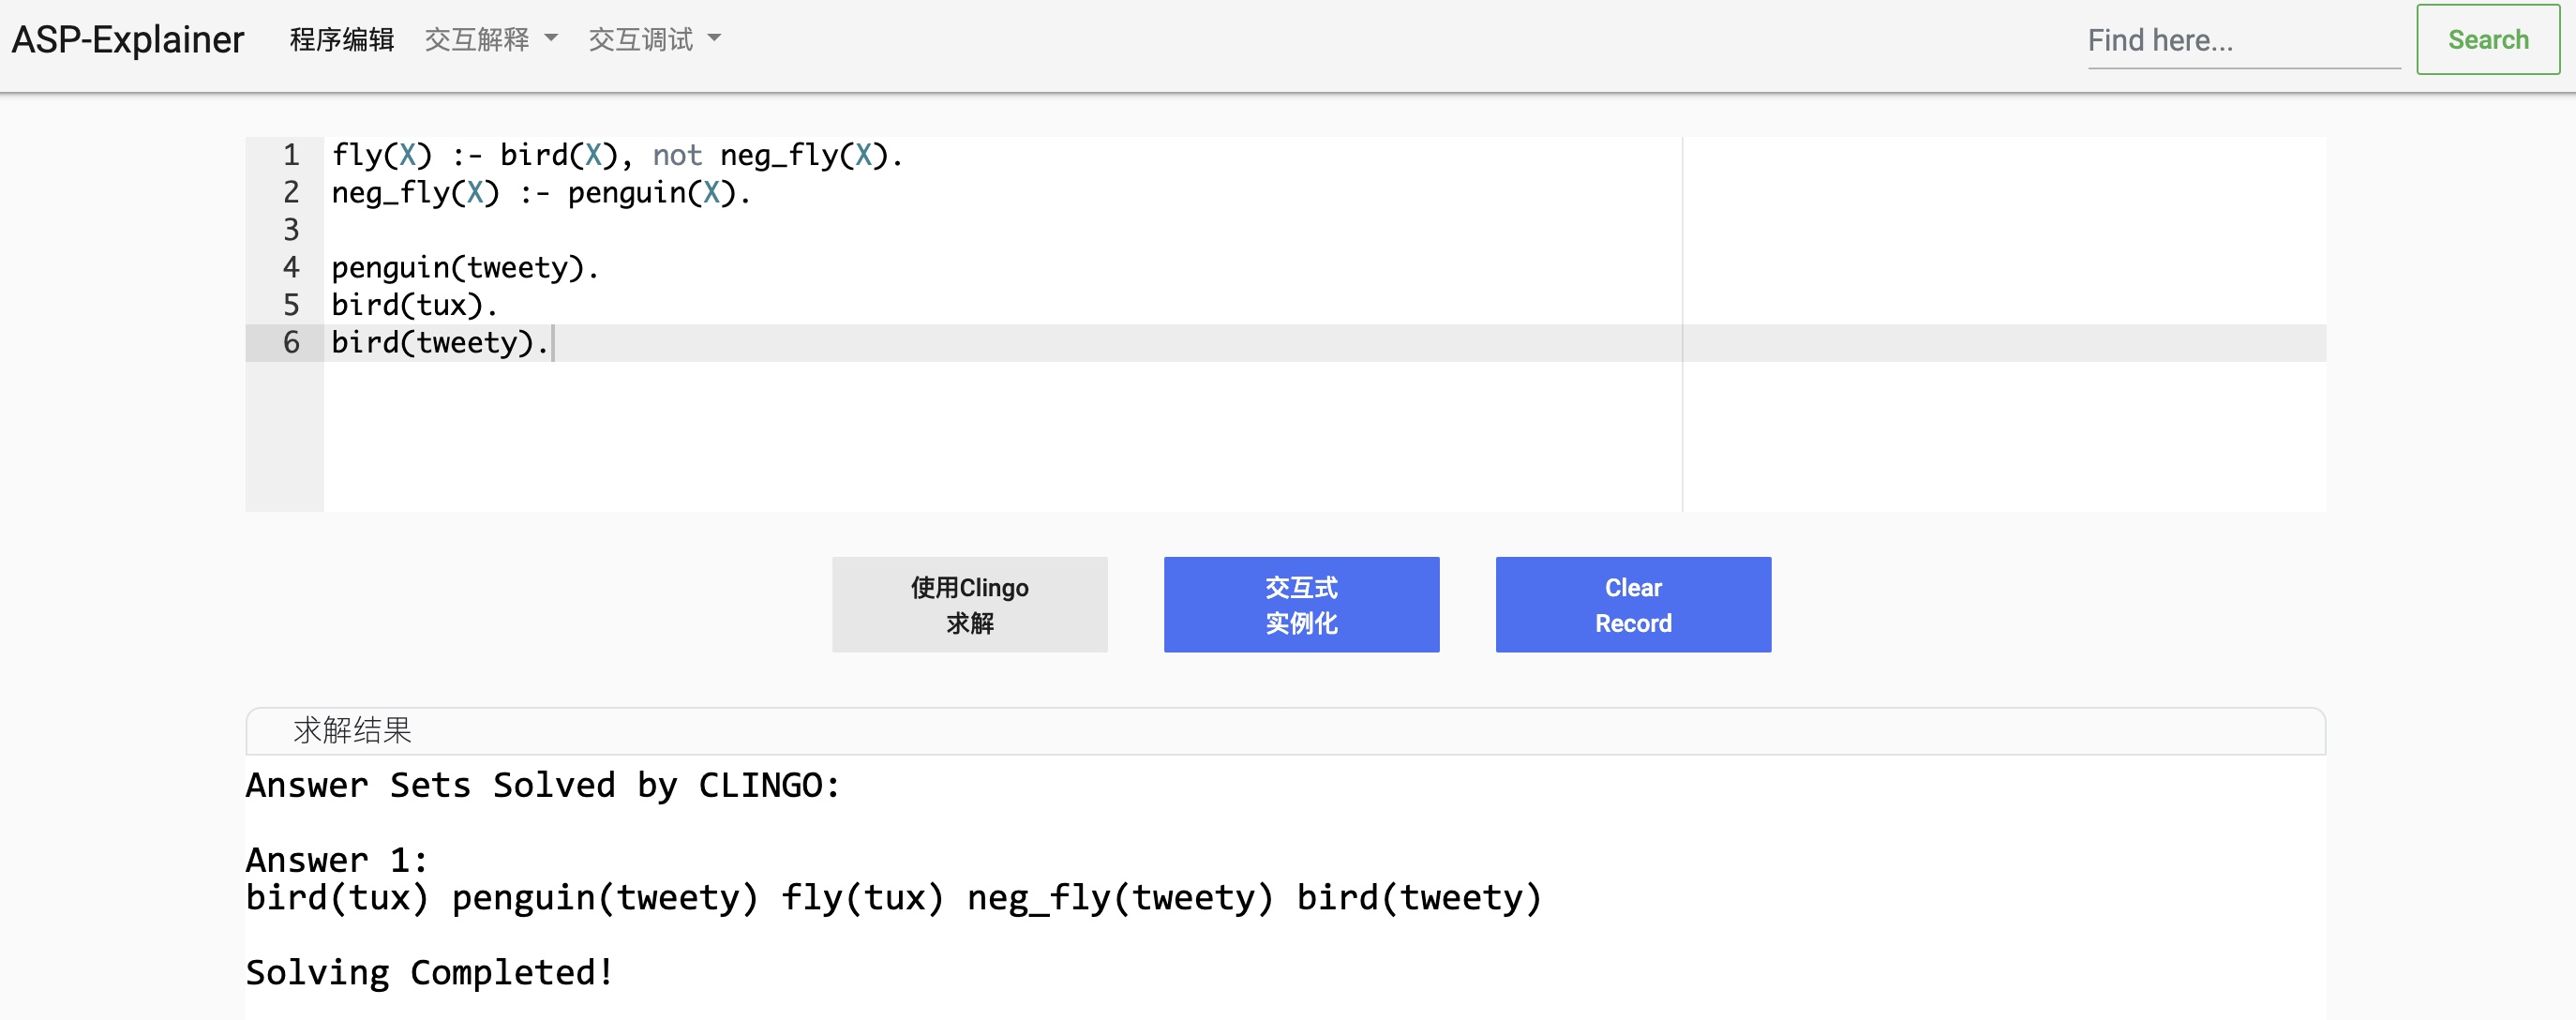
\includegraphics[width=0.8\linewidth]{figures/程序录入.jpg}
    \caption{程序录入与求解界面}
    \label{fig:prginput}
\end{figure}

程序录入与求解模块的功能如图\ref{fig:prginput}所示,该模块用于接收用户待解释的逻辑程序。当用户点击按钮\textbf{“使用Clingo求解”}时,前端将向后端发送GET请求,参数为用户输入的字符串为逻辑程序,后端收到逻辑程序字符串后,将对程序字符串进行语法解析,从程序中提取规则,进一步从规则中提取正、负体部及正负体部中的文字,特别是进行重要项的提取:包括变量、常量等,并存放入数据库中,以方便后续对程序进行实例化。

\subsubsection*{2) 程序交互式实例化}
当完成程序录入与求解后,将通过向用户进行交互式实例化,如图\ref{fig:prggrding}所示。首先,用户勾选$bird(X)$,表示在解释的过程中,认为所有与$bird$相关的文字默认为真,即不会寻求“为什么bird(a)为假”的解释。紧接着,对其他文字中的变量进行变量绑定,例如$fly(X)$中的$X$与$bird(X)$中的$X$进行绑定,含义为“若$X$满足$fly(X)$,则$X$也满足$bird(X)$”。

\begin{figure}
    \centering
    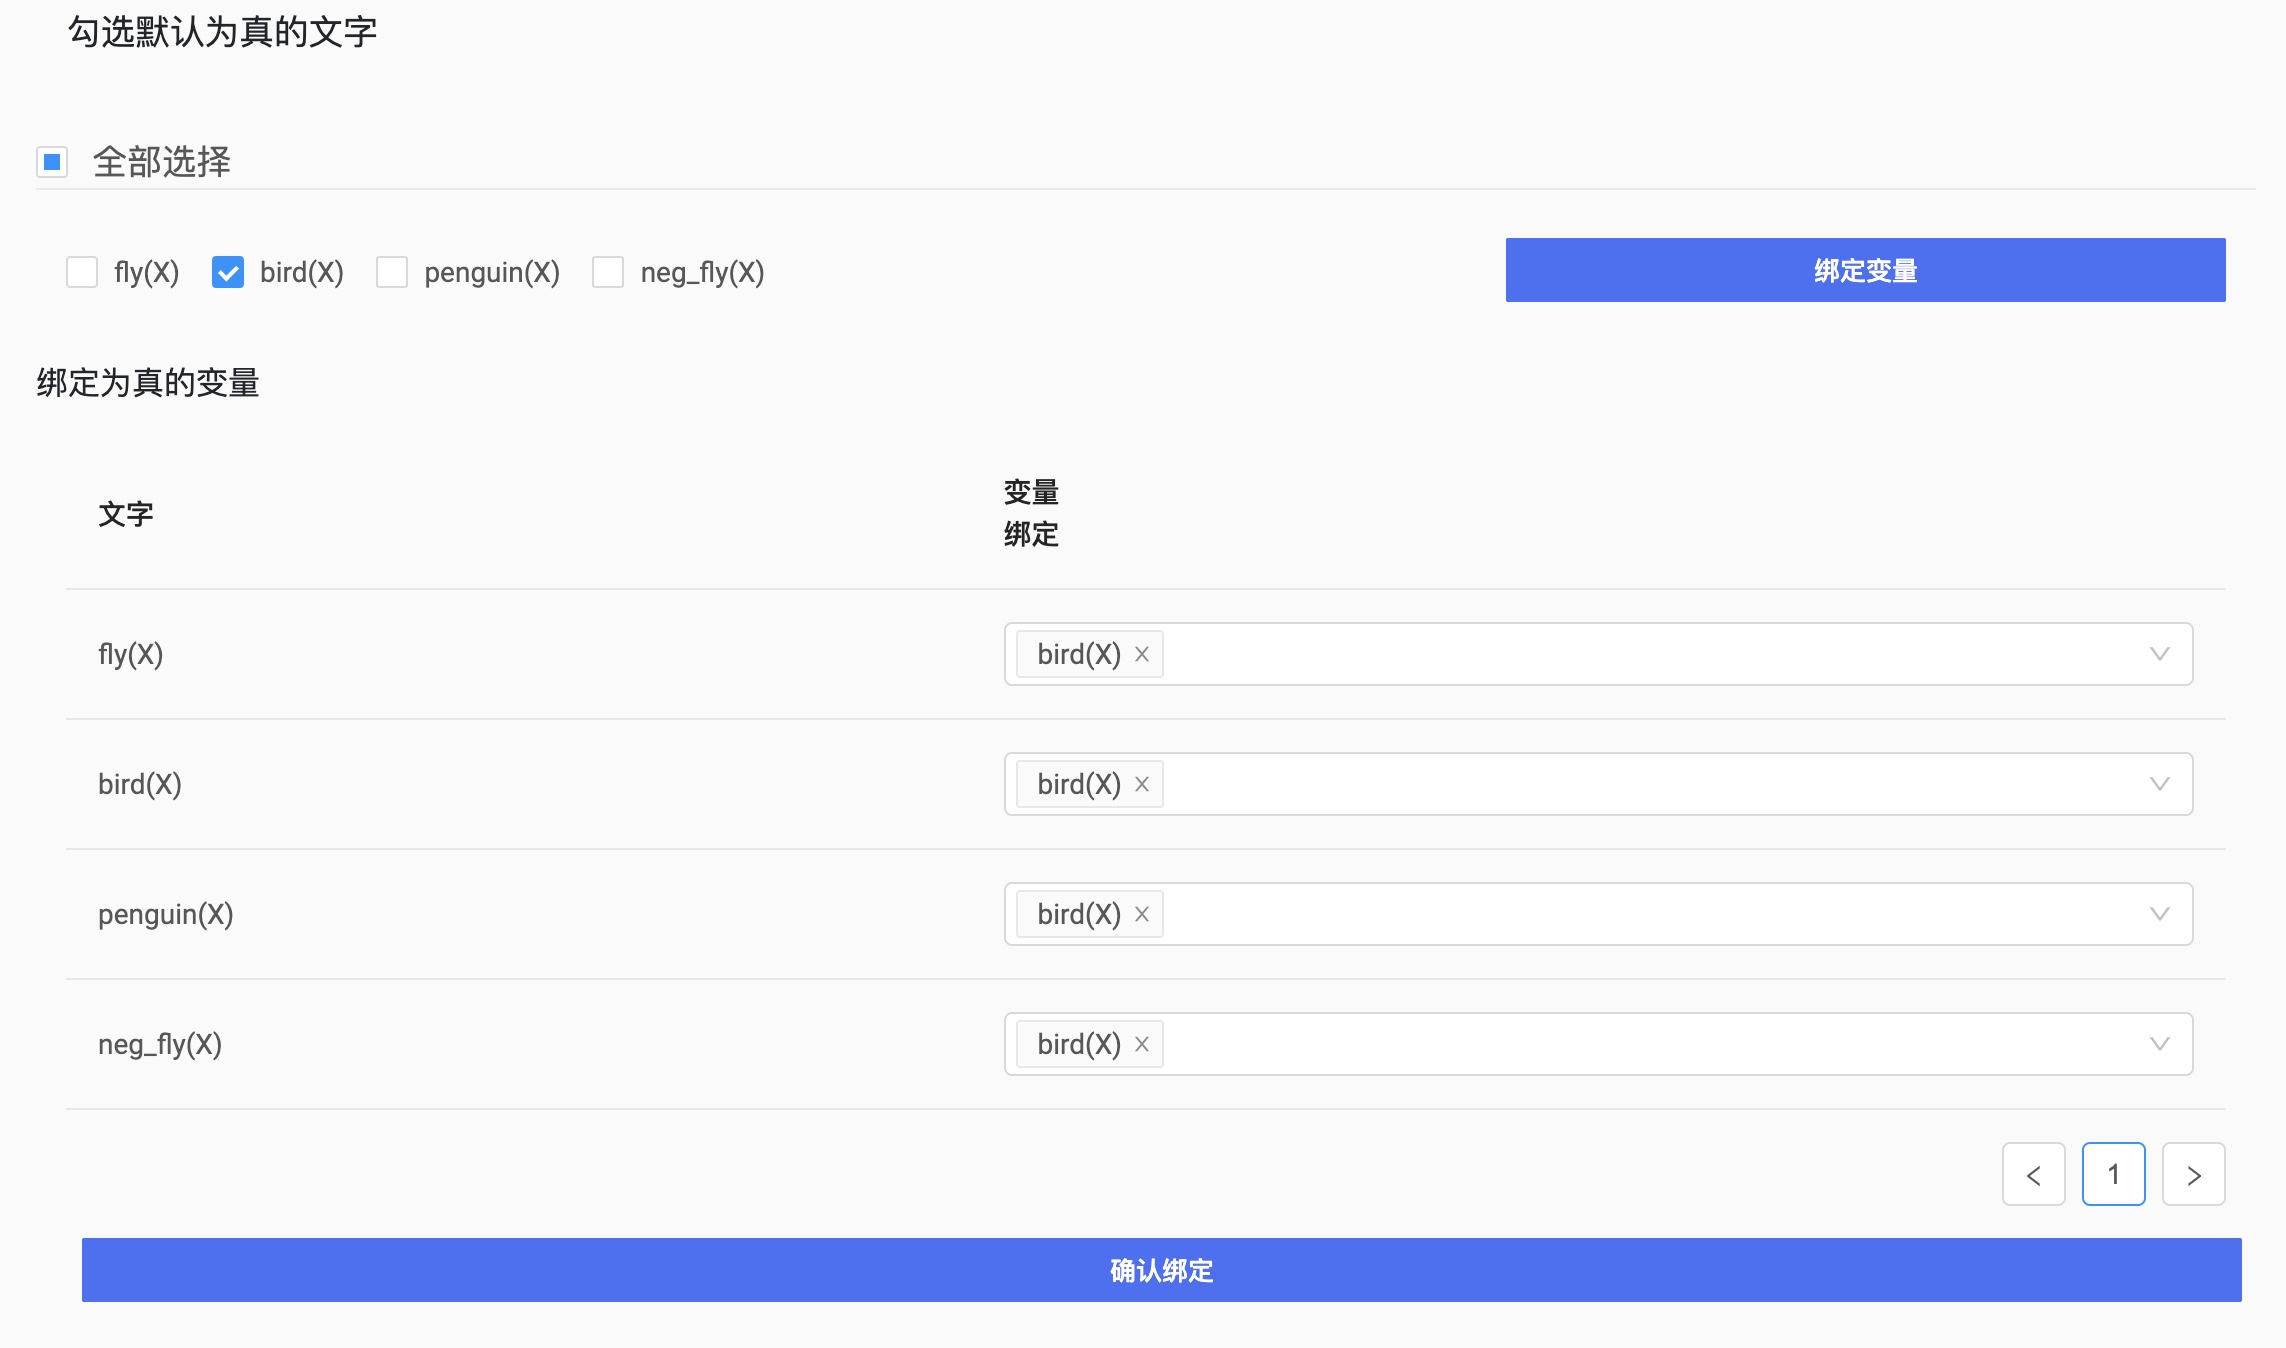
\includegraphics[width=0.8\linewidth]{figures/实例化交互.jpg}
    \caption{程序交互式实例化界面}
    \label{fig:prggrding}
\end{figure}

绑定结束后,后端将进行程序实例化工作,得到完整的实例化程序,如图\ref{fig:prggrdingoutput}所示。

\begin{figure}
    \centering
    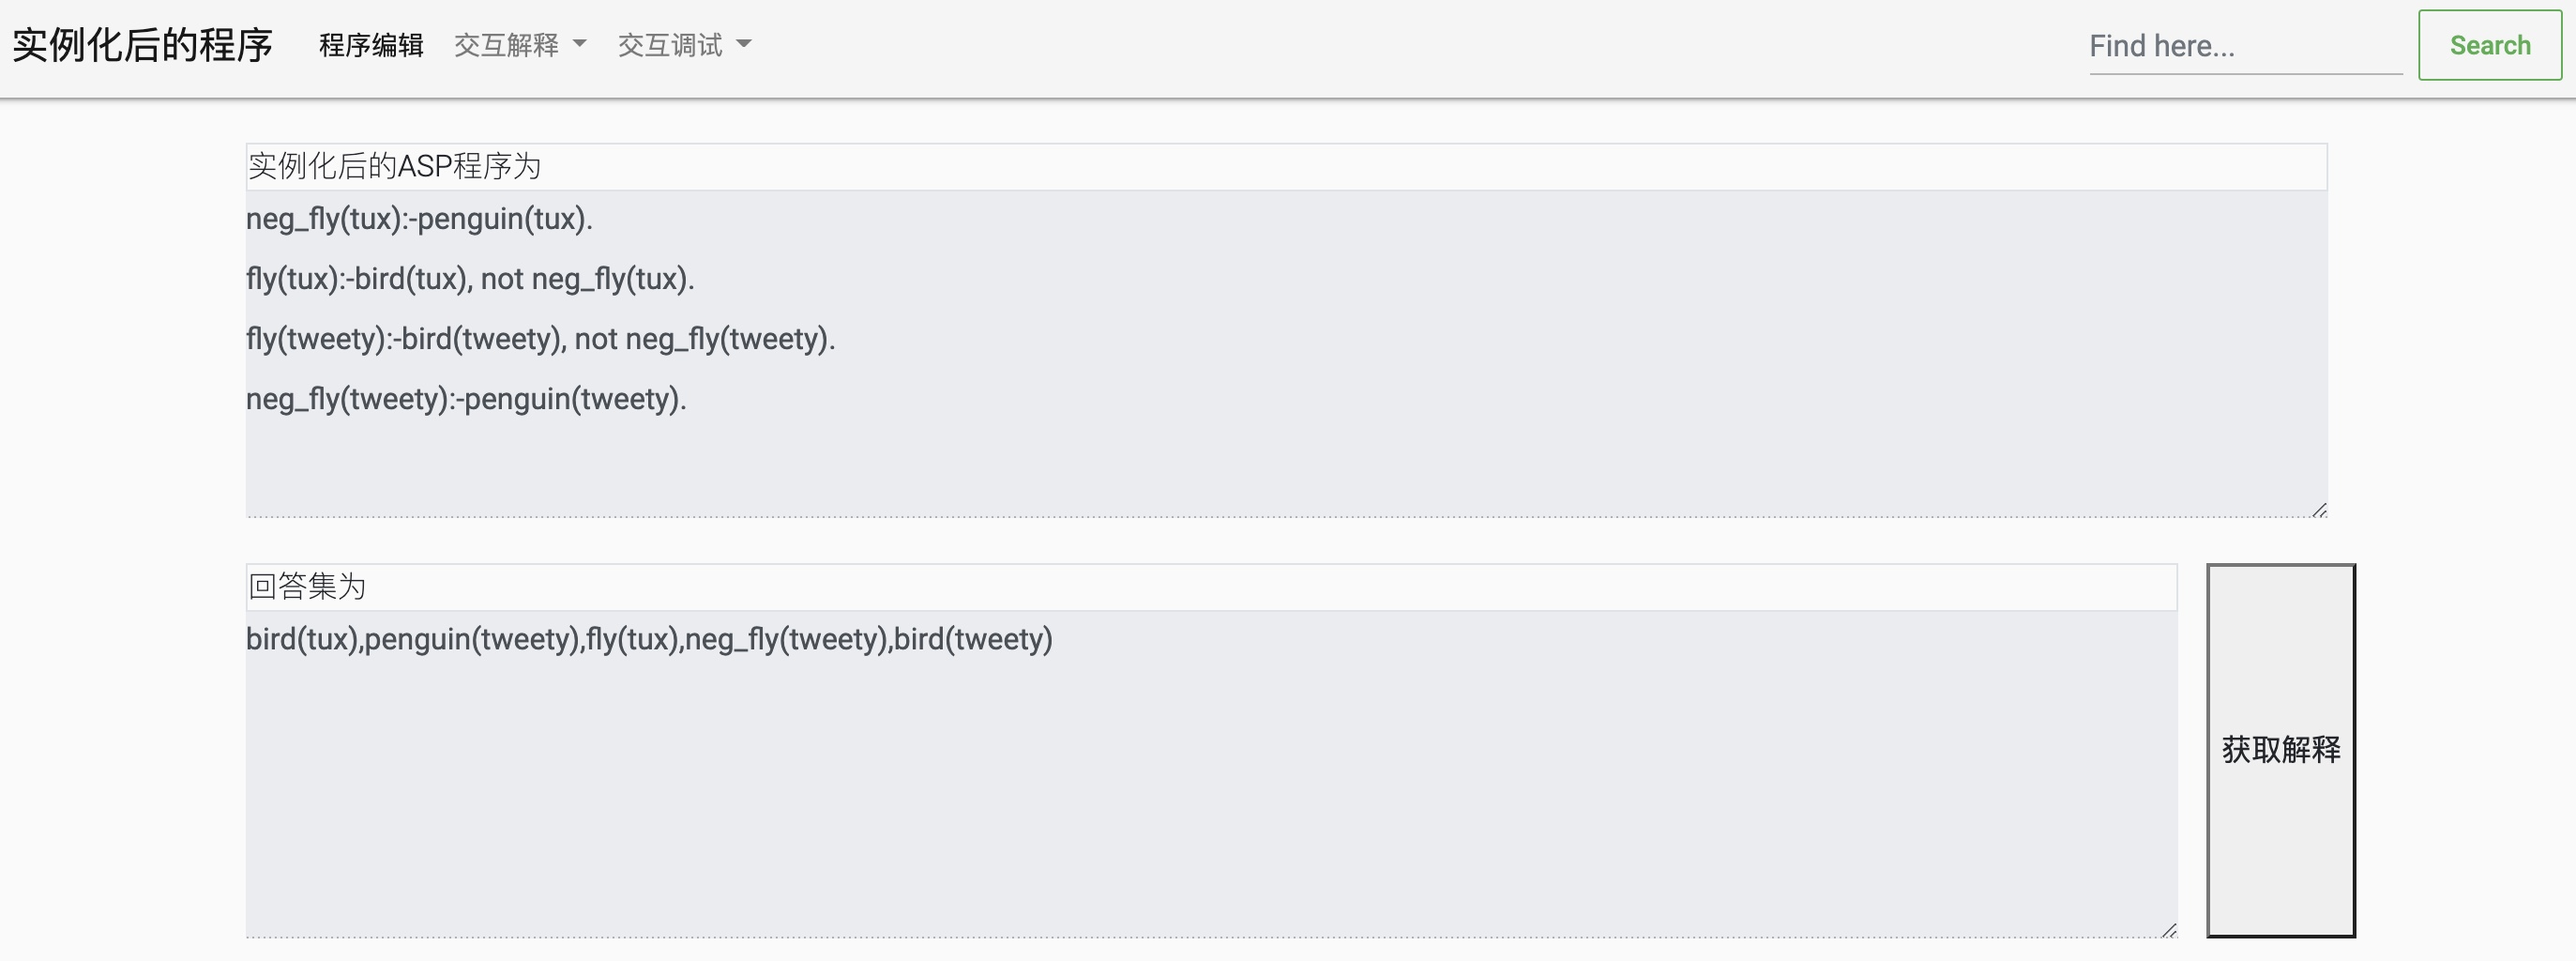
\includegraphics[width=0.8\linewidth]{figures/实例化结果.jpg}
    \caption{程序交互式实例化结果展示界面}
    \label{fig:prggrdingoutput}
\end{figure}

\subsubsection*{3) 解释交互展开}
在交互式实例化结果展示界面,用户点击获取解释,即可选择对应的回答集查看解释结果。对于仅有一个回答集的程序,用户首先选择待解释的回答集中的文字,解释图中将展示该文字在解释空间中的文字结点,如图\ref{fig:littoselect}所示,图中选择了$fly(tux)$。
\begin{figure}[htbp]
    \centering
    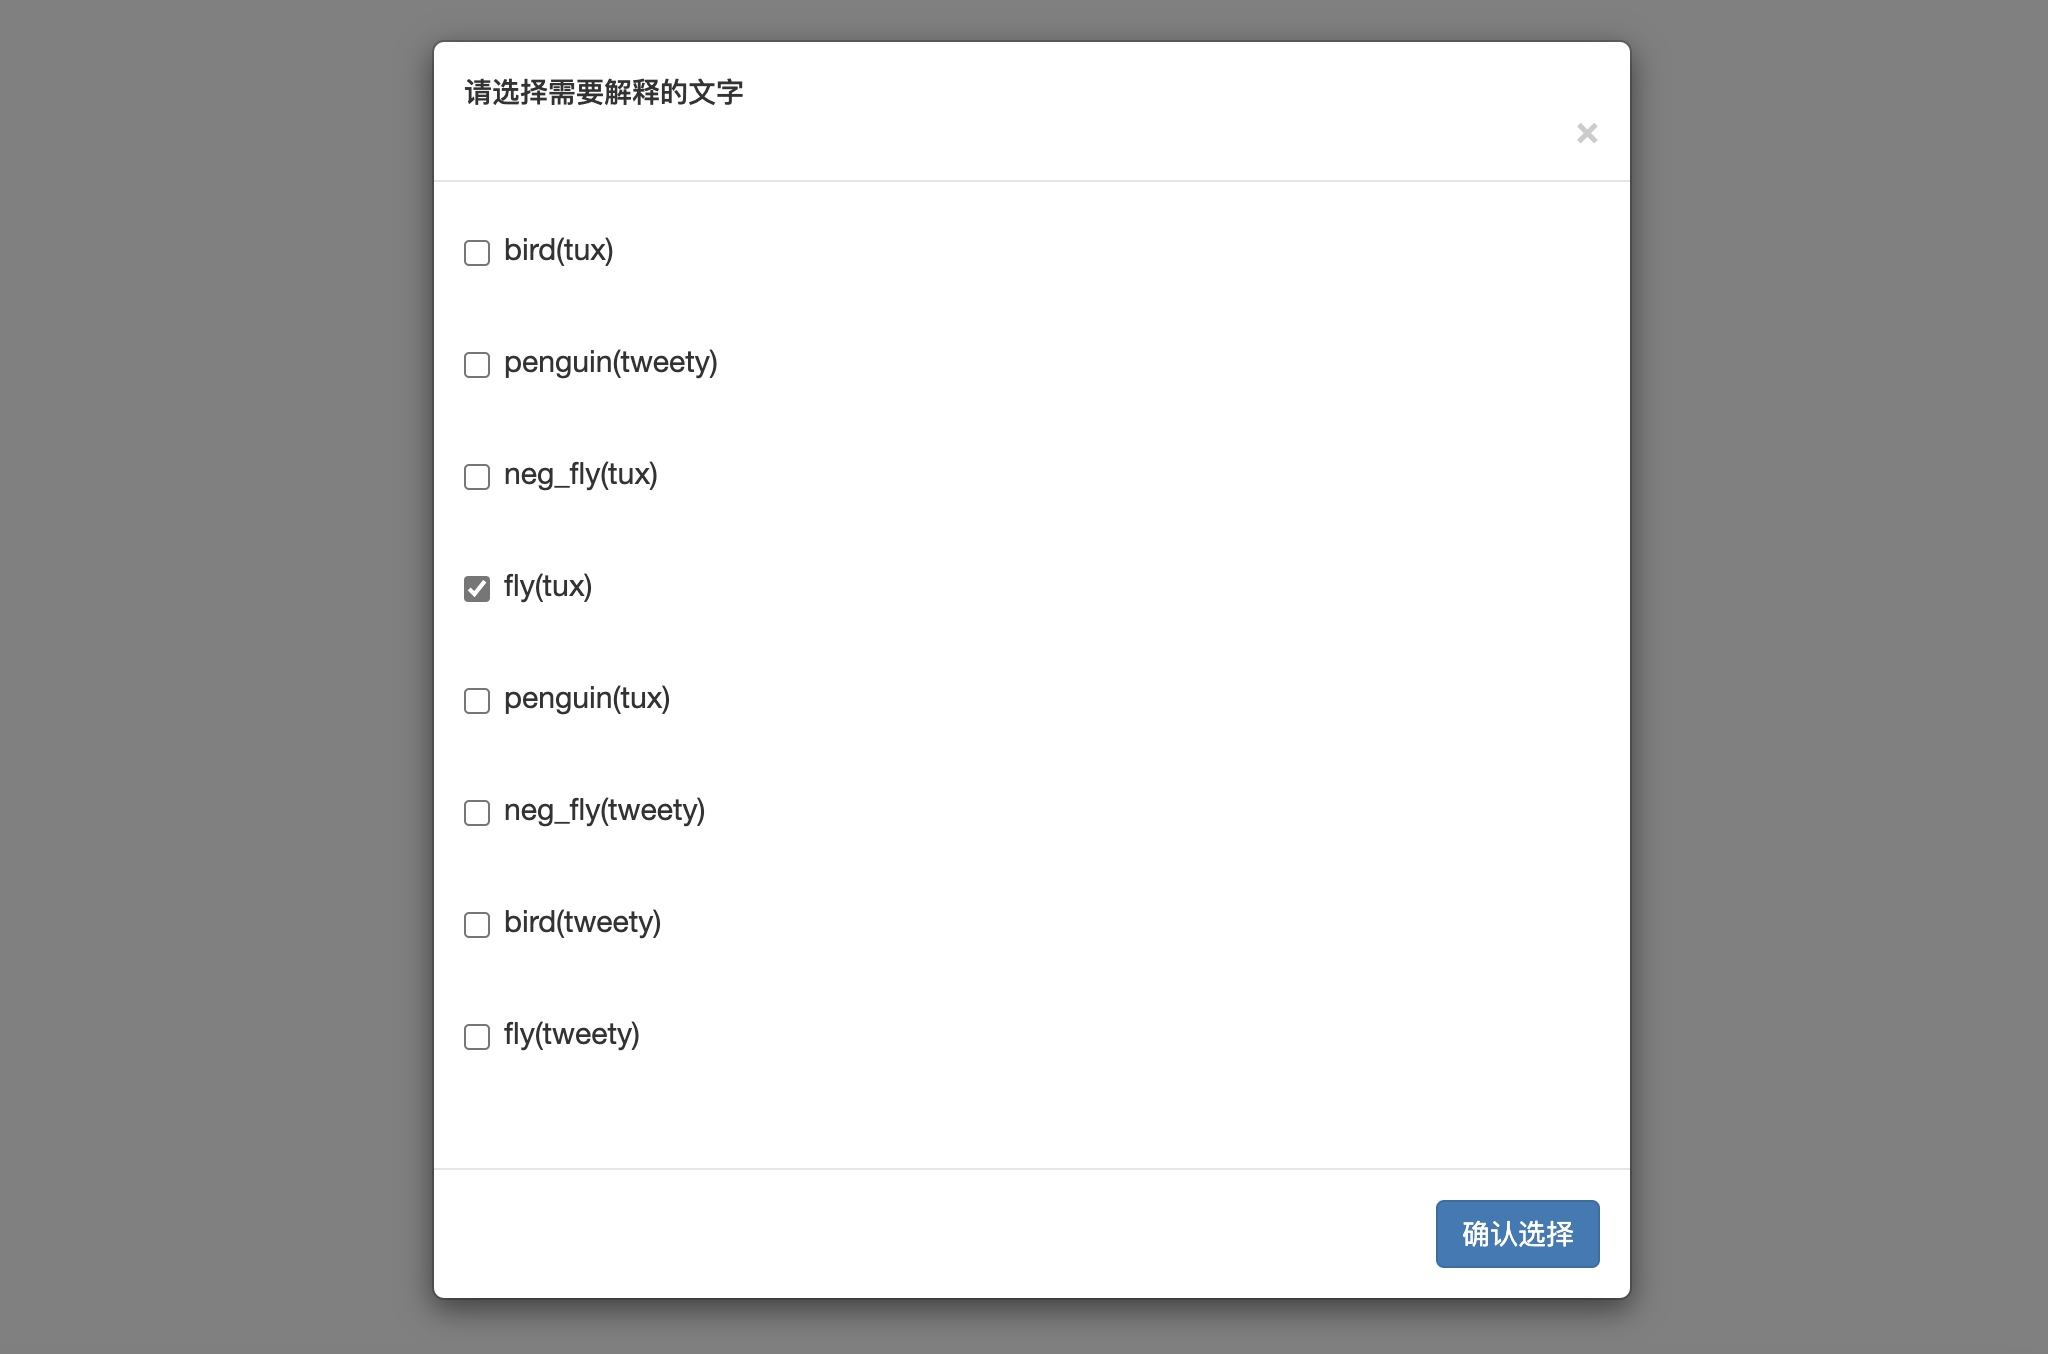
\includegraphics[width=0.8\linewidth]{figures/待解释文字选择.jpg}
    \caption{待解释文字选择界面}
    \label{fig:littoselect}
\end{figure}

在双击该待解释结点之后,将会弹出可选的下一级的可选结点,供用户选择,如图\ref{fig:expandNodeSelect}所示,选中$neg\_fly(X)$后,展开的结果如图\ref{fig:expandResult}所示。
\begin{figure}[htbp] 
    \centering 
    \begin{minipage}[t]{0.48\textwidth} 
        \centering 
        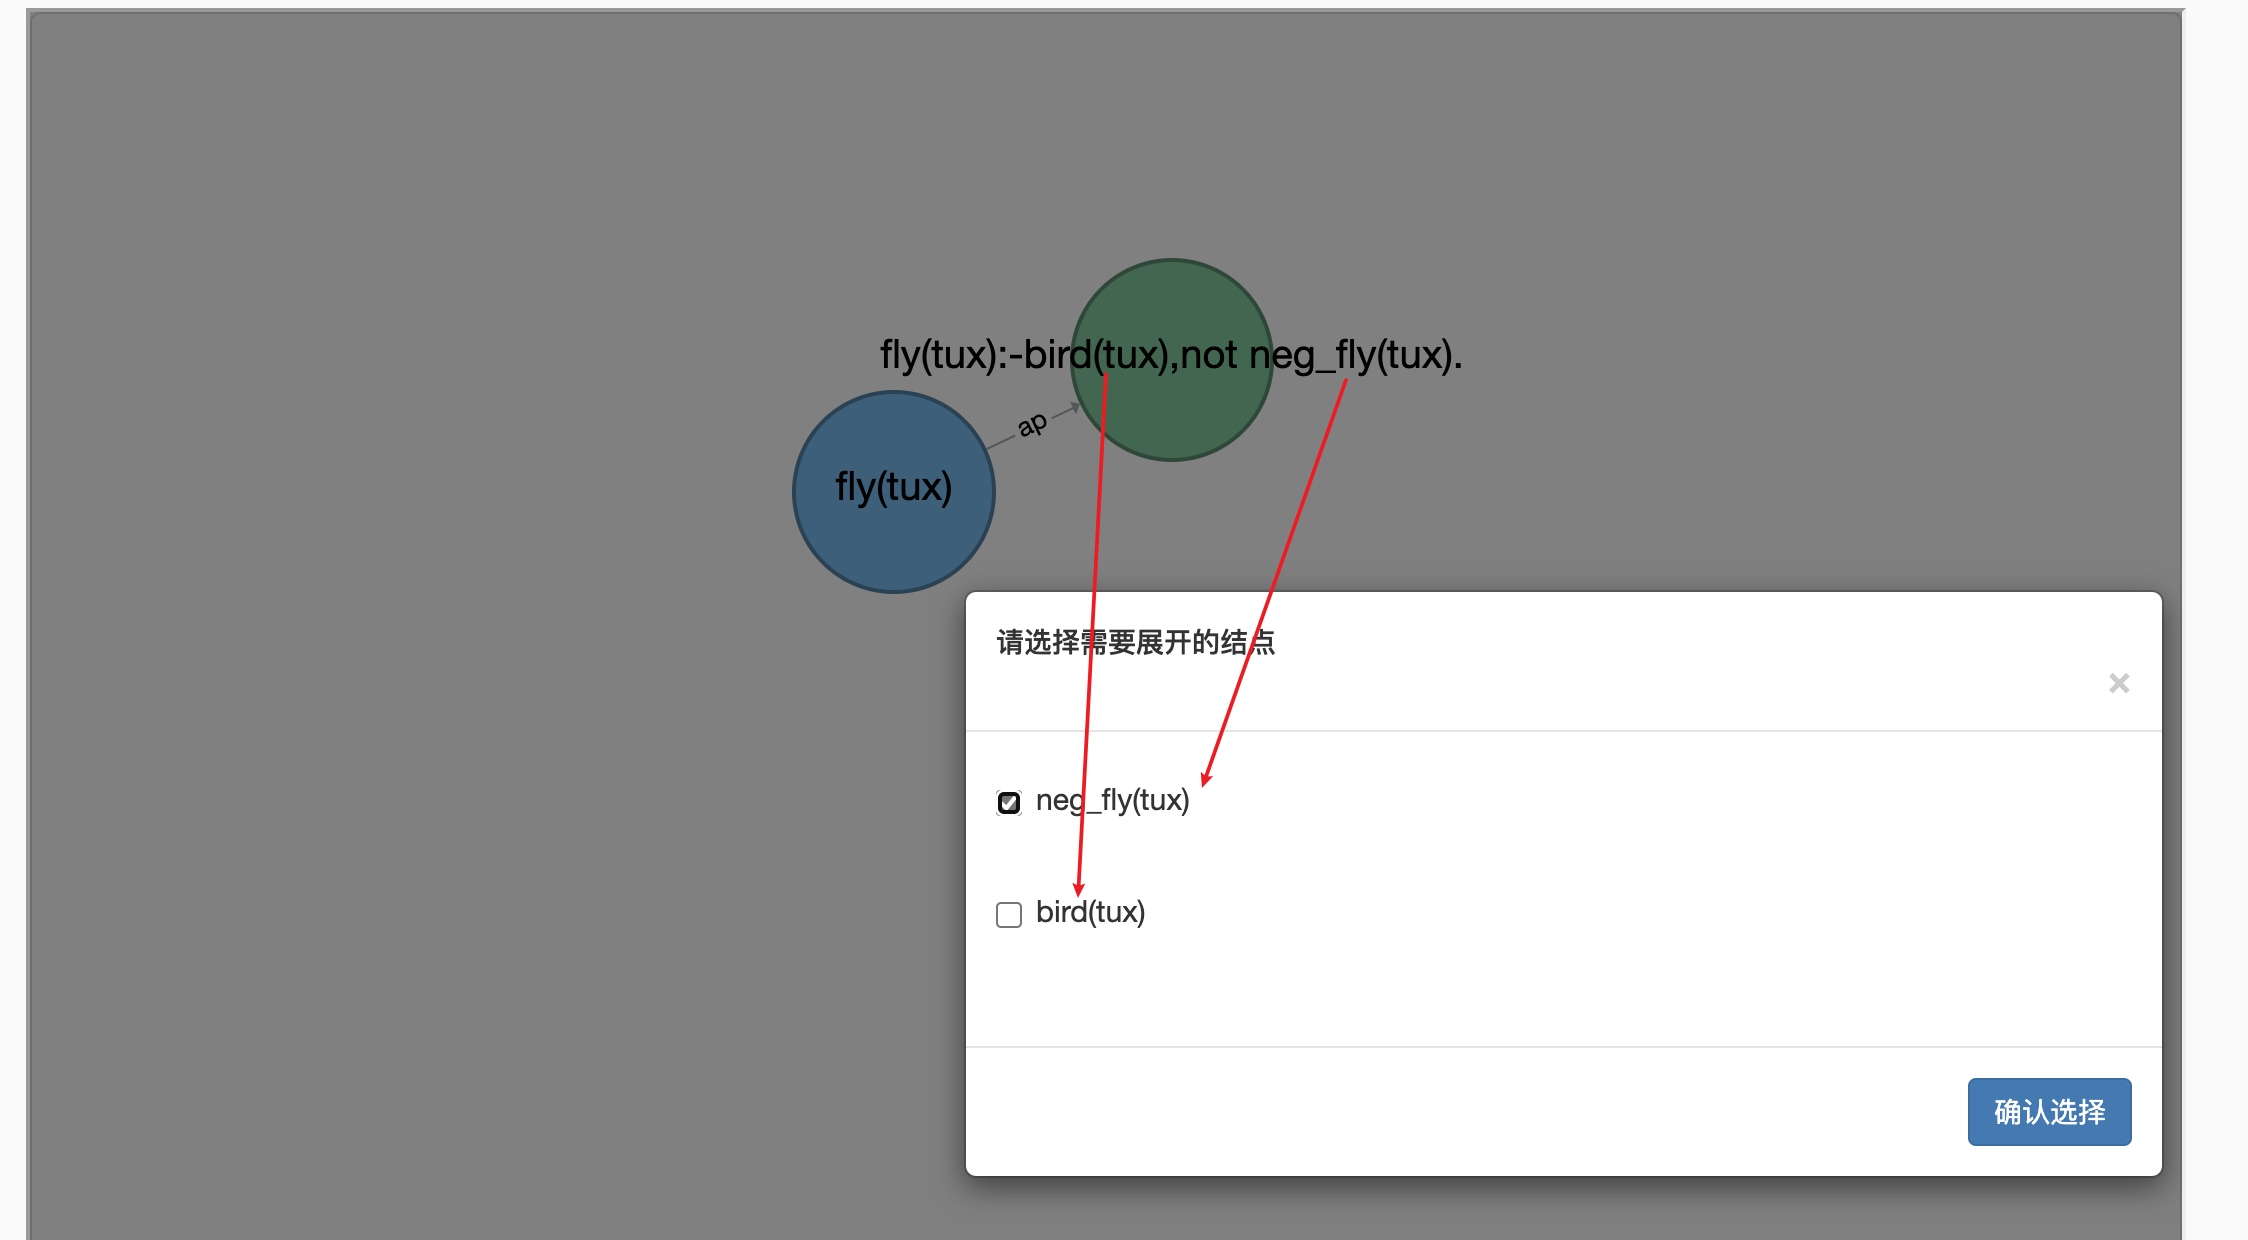
\includegraphics[width=\linewidth]{figures/具体展开.jpg} 
        \caption{规则结点展开选择界面} 
        \label{fig:expandNodeSelect} 
    \end{minipage} 
    \begin{minipage}[t]{0.48\textwidth} 
        \centering 
        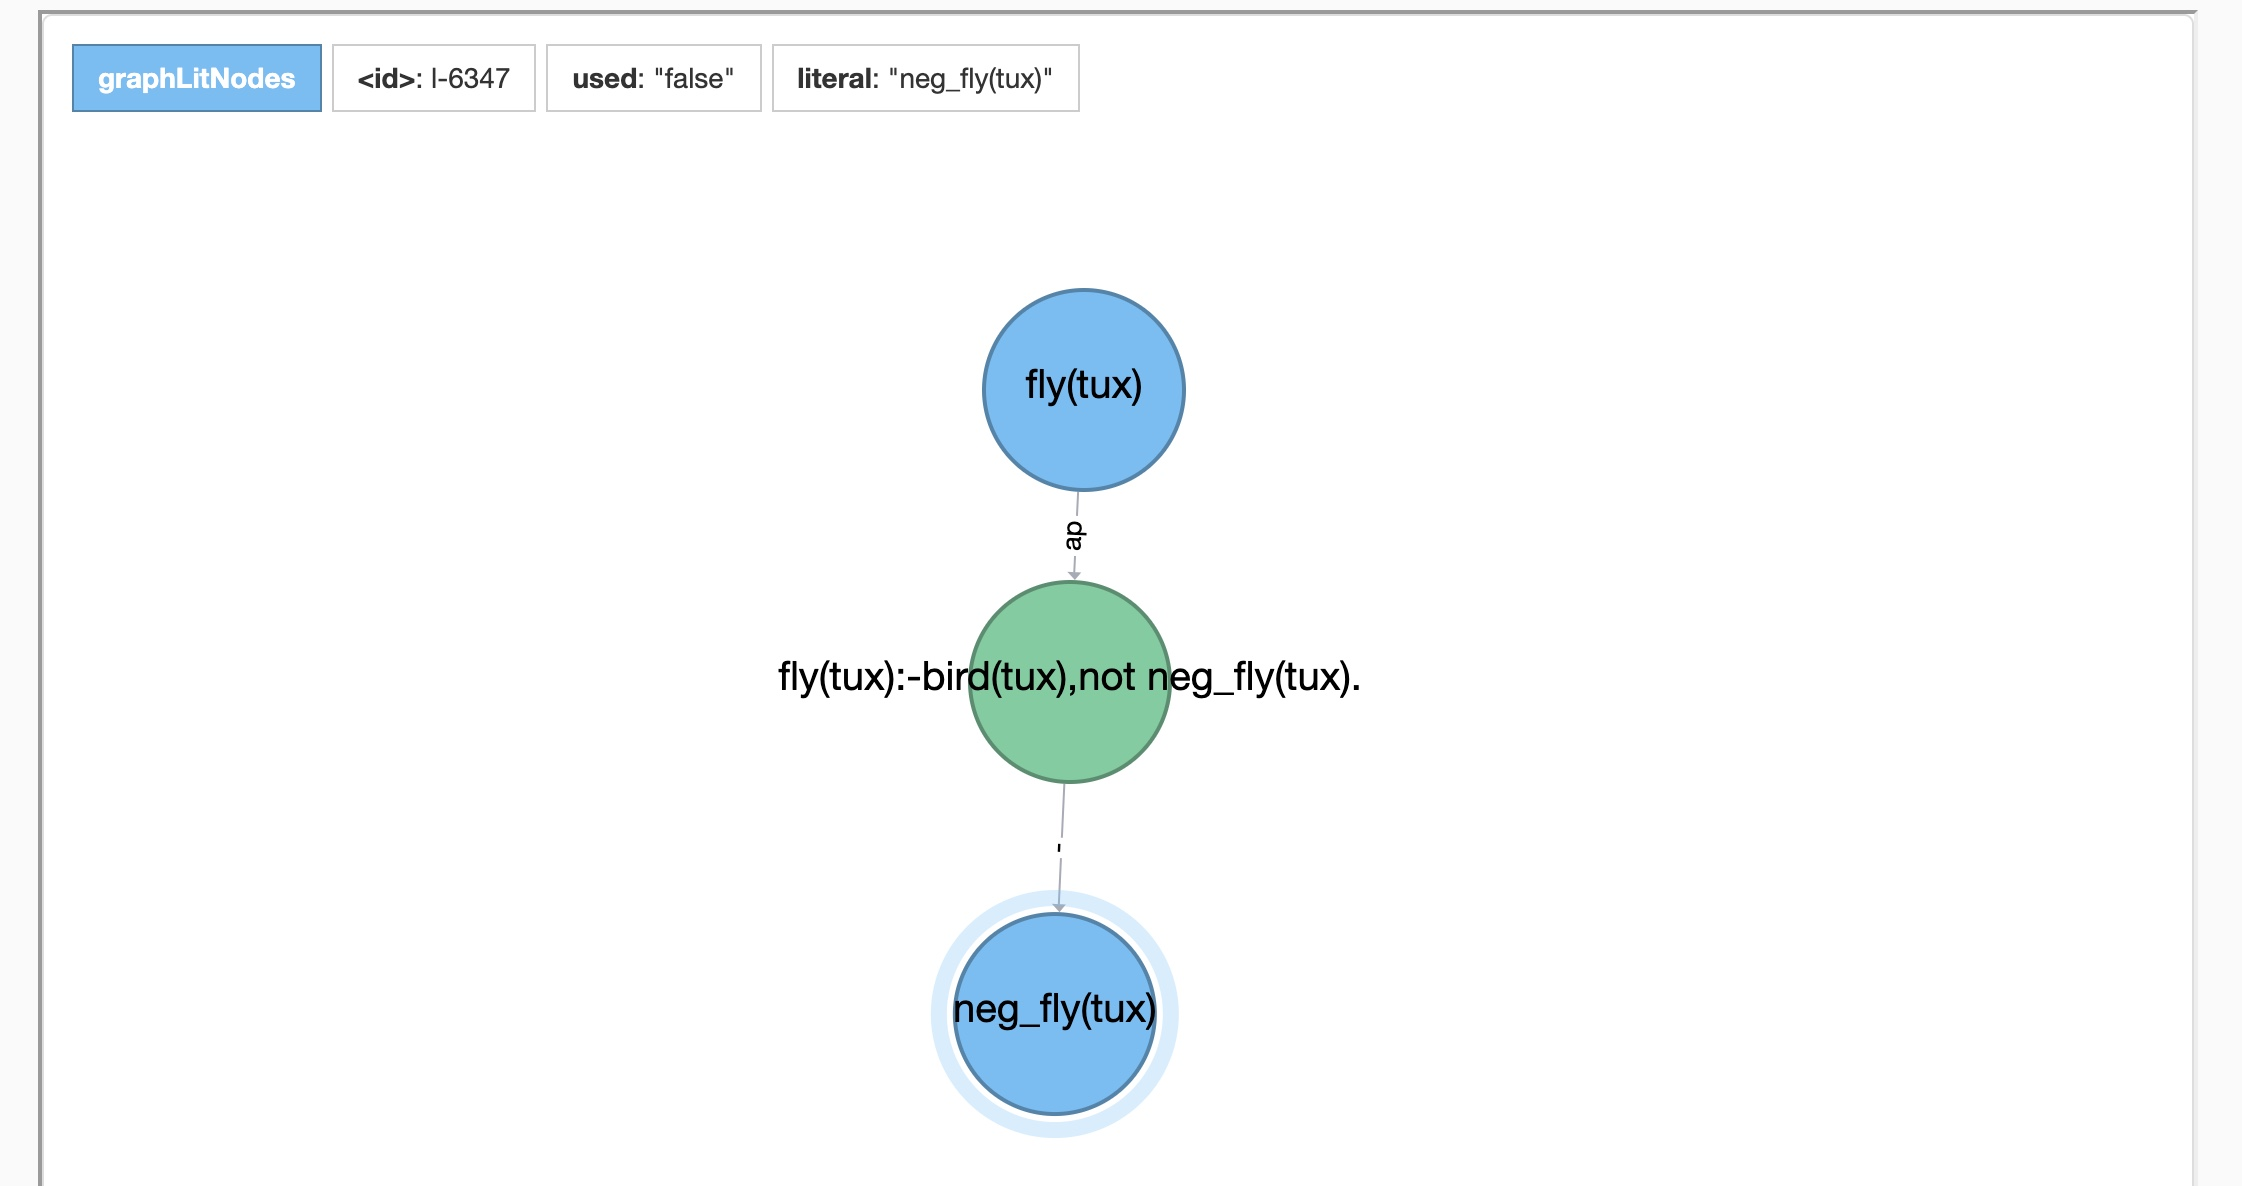
\includegraphics[width=\linewidth]{figures/文字展开结果.jpg} 
        \caption{规则结点展开结果} 
        \label{fig:expandResult} 
    \end{minipage} 
\end{figure}

按照各步骤逐层展开,得到的完整解释图界面如图\ref{fig:completeexp}所示。图中,蓝色结点为文字结点,绿色结点为规则结点,红色结点为终结结点。图\ref{fig:completeexp}解释了为何tux能飞,并且给出了完整的解释图。
\begin{figure}[htbp]
    \centering
    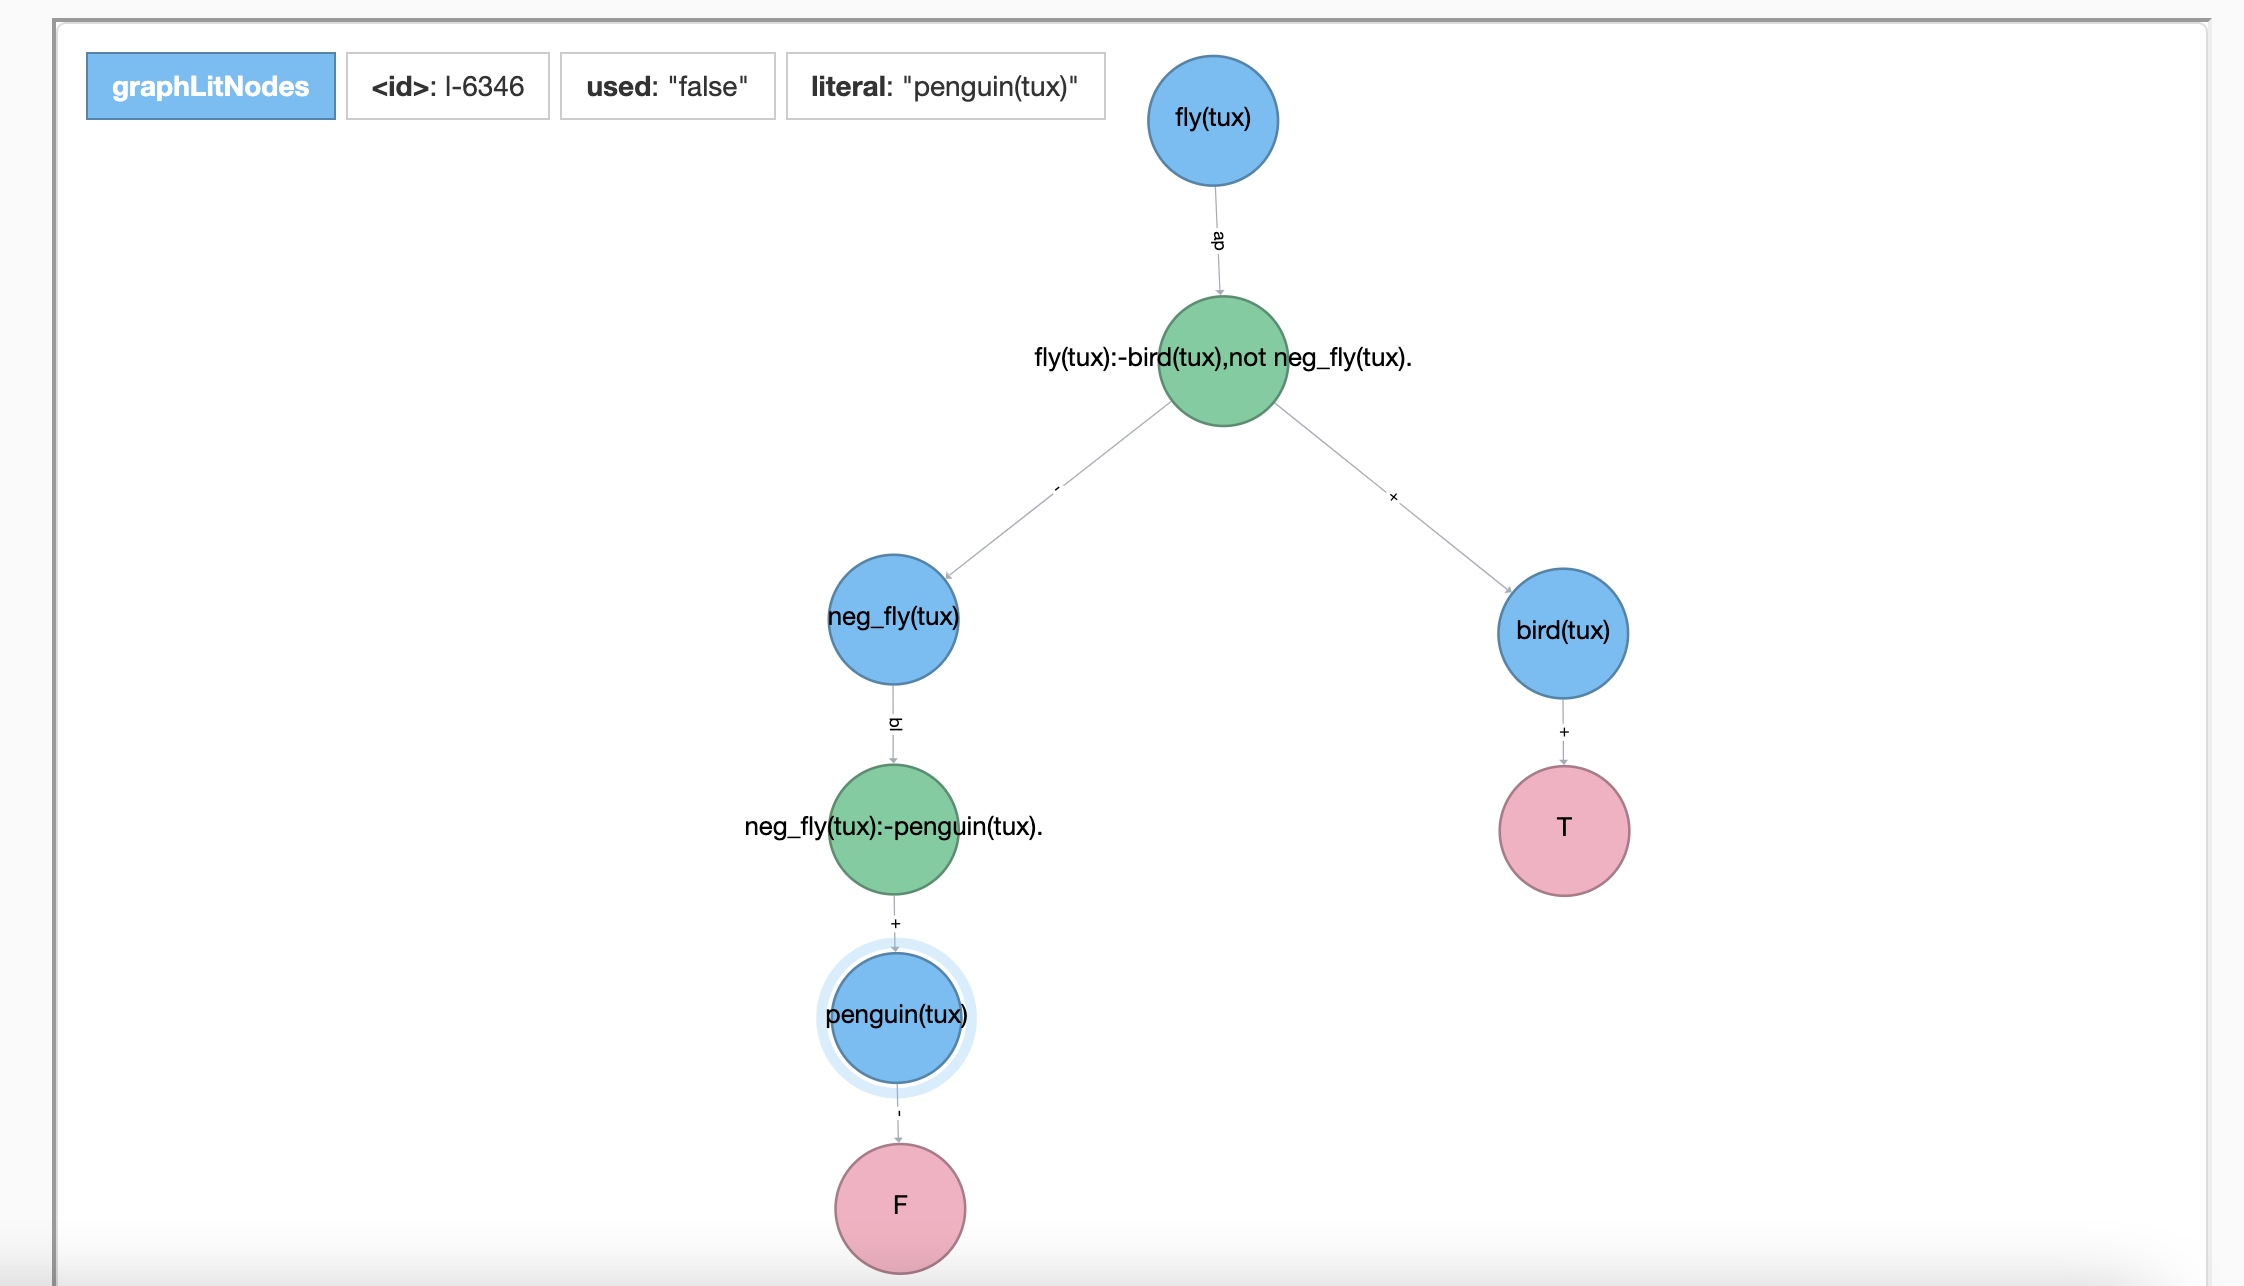
\includegraphics[width=0.8\linewidth]{figures/完整解释图.jpg}
    \caption{完整解释图}
    \label{fig:completeexp}
\end{figure}

% todo:调试界面设计与展示

\section{实例分析}


\section{本章小结}
